\begin{figure}
\centering
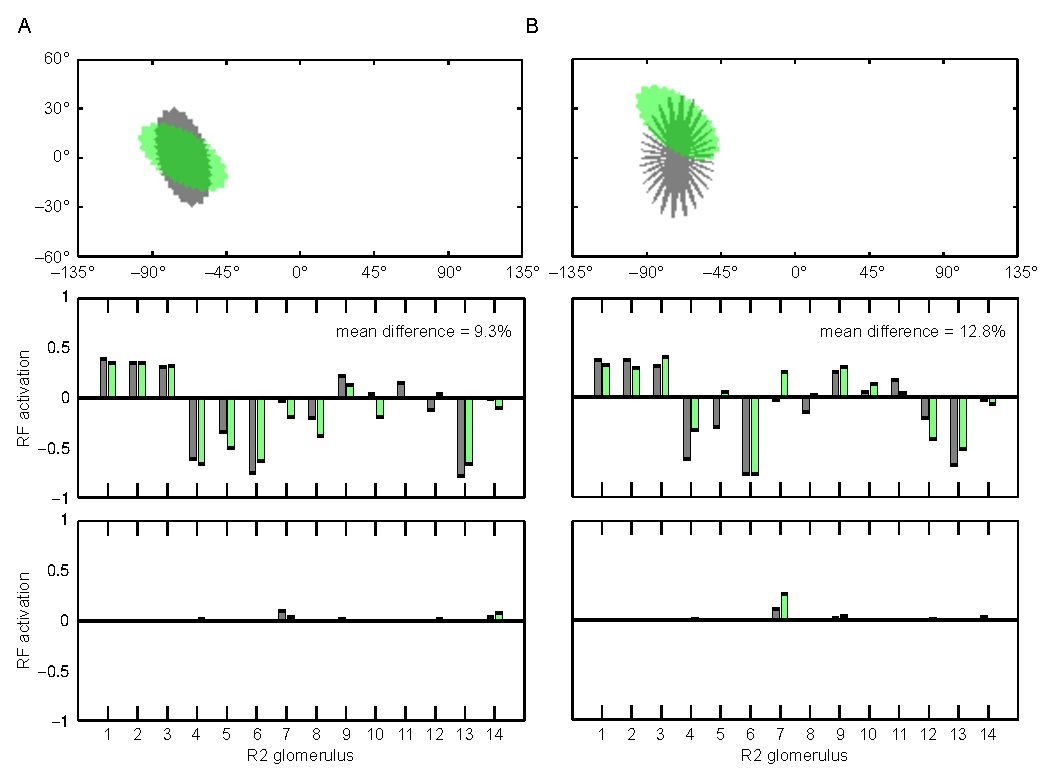
\includegraphics{figures/simdiff}
\caption{R2 cells do not encode detailed shape information.
The apparent difference between visual stimuli does not always correspond to with ring neuron outputs.
The stimuli here are `blobs' of the form described previously (in Methods).
An optimisation was performed in Matlab (\texttt{fminsearch} function) to minimise the ratio of blob difference to difference in activation (A) or its inverse (B).
Pairs of stimuli are shown in grey and green (top; in the simulation both are black).
The corresponding activations of separate (left-hemispheric) R2 glomeruli are shown at the bottom.
A: Two similar patterns give a mean difference in activity of 9.3\%.
B: Two very different patterns with different centres of mass (0\degree\ and 20\degree) give a mean difference in activity of 12.8\%.
}

\label{fig:fcp}
\end{figure}